\documentclass[../main.tex]{subfiles}
\begin{document}
	\begin{theorem}[LDU -- разложение]\ \\
		$\forall k = 1 \ldots n - 1 \Space \triangle _k \neq 0 \Leftrightarrow $ \belowbaseline[-14pt]{$\begin{matrix}
				\exists ! L \text{ унитарная нижняя матрица}\\
				\exists ! U \text{ унитарная верхняя матрица}\\
				\exists ! D = diag(\alpha_1 \ldots \alpha_k) \\
				\boxed{A = LDU} \Space \alpha_i \neq 0 \; \; i = 1 \ldots n - 1
			\end{matrix}$}\n 
		$A = \underset{\stackrel{\uparrow}{\text{нижнетр.}}}{L}\ \underset{\stackrel{\uparrow}{\text{верхнетр.}}}{U}$ неоднозначн. (не обязательно унитреугольные)
	\end{theorem}
	\begin{proof}
		$(\Leftarrow)\n 
		A = LDU \n 
		det A =\underset{=1}{det L} \ det D \ \underset{=1}{det U} = d_1 d_2 \ldots d_{n-1} d_n$\n 
		\underline{Докажем: } $\begin{matrix}
			A_k = L_k D_k U_k \\
			\triangle_k = det A_k
		\end{matrix} \Space \; \; L = \begin{pmatrix}
			1 & & 0 \\
			& \ddots\\
			* & & 1
		\end{pmatrix} \Space U = \begin{pmatrix}
			1 & & *\\
			& \ddots \\
			0 & & 1
		\end{pmatrix} \Space A_k = \begin{pmatrix}
			a_{11} & \ldots & a_{1k} \\
			\ldots\\
			a_{k1} & \ldots & a_{kk}
		\end{pmatrix} \n 
		A = LDU \Leftrightarrow a_{ij} = \sum\limits_{s=1}^n \sum\limits_{t=1}^n \underset{\begin{matrix}
				||\\
				0\\
				s>i
			\end{matrix}}{l_{is}} d_{st} \underset{\begin{matrix}
				||\\0\\t>j
			\end{matrix}}{u_{tj}} = $\belowbaseline[-18pt]{$\begin{matrix}
			\sum\limits_{s=1}^i \sum\limits_{t=1}^j l_{is} d_{st} u_{tj}\n 
			1 \leq i, j \leq k \\
			\Updownarrow\\
			(L_k D_k U_k)_{ij}
	\end{matrix}$}\n 
	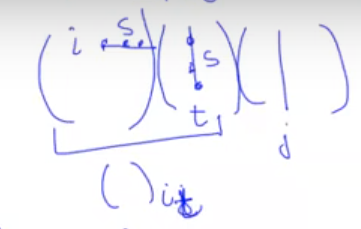
\includegraphics[width=130px]{pic29} 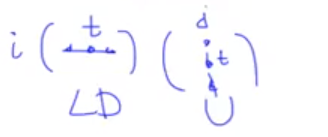
\includegraphics[width=130px]{pic30}\n 
	$\triangle_k = det A_k = \underset{=1}{det L_k} \ det D_k \ \underset{=1}{det U_k} = det D_k = d_1 \ldots d_k \n 
	\triangle_k \neq 0 \; \; \; k = 1 \ldots n-1 \Space d_k \neq 0 \n 
	\boxed{d_k = \mathlarger{\frac{\triangle_k}{\triangle_{k-1}}}} \begin{matrix}
		k = 1 \ldots n \\
		\triangle_0 = 1
	\end{matrix} \n 
	(\Rightarrow) \underset{\neq 0 }{\triangle_1} \ldots \underset{\neq 0}{\triangle_{n-1}}$\n
	\underline{М.м.и.}
	\begin{mylist}
		\item база $ n= 1 \; \; \triangle_1 \neq 0  \Space a_{11} = \underset{=L}{1} \cdot \underset{=d_1}{a_{11}} \cdot \underset{=U}{1}$
		\item Инд. предпол: $\pu$ верно для $n = k \Space \triangle_1 \neq 0 \ldots \triangle_k \neq 0 \n 
		A_k = L_k D_k U_k$ единств. образом $D_k = diag (d_1 \ldots d_k) \n 
		d_i \neq 0 \; \; i = 1 \ldots k$
		\item Инд. переход: $n = k+1$ ? \n 
		$A_{k+1} = \begin{pmatrix}
			A_k & \vline& b_{k+1} \\
			\hline
			C_{k+1} & \vline&
			 d_{k+1 \ k+1}
		\end{pmatrix} \Space L_{k+1} = \begin{pmatrix}
			L_k & \vline & 0 \\
			\hline 
			x & \vline & 1
		\end{pmatrix} \Space U_{k+1} = \begin{pmatrix}
			U_k & \vline & y \\
			\hline
			0 & \vline & 1
		\end{pmatrix} \n 
		D_{k+1} = diag(d_1 \ldots d_k d_{k+1})\n 
		\underline{A_{k+1} = L_{k+1} D_{k+1} U_{k+1}} \Space x, y, d_{k+1}?$ и единств?\n 
		$A_{k+1} = \underbracket{\begin{pmatrix}
				L_k & \vline & 0\\
				\hline 
				x & \vline & 1
			\end{pmatrix} \begin{pmatrix}
				D_k & \vline & 0 \\
				\hline 0 & \vline & d_{k+1}
			\end{pmatrix}}_{\begin{pmatrix}
				L_k D_k & \vline & 0 \\
				\hline x D_k & \vline & d_{k+1}
			\end{pmatrix}} \begin{pmatrix}
			U_k & \vline & y \\
			\hline 0 & \vline & 1
	\end{pmatrix} = \begin{pmatrix}
		\boxed{L_k D_k U_k} & \vline & L_k D_k y \\
		\hline x D_k U_k & \vline & x D_k y + d_{k+1}
	\end{pmatrix} = \begin{pmatrix}
		\boxed{A_k} & \vline & b_{k+1} \\
		\hline c_{k+1} & \vline & a_{k+1 \ k+1}
	\end{pmatrix} \n 
	\Leftrightarrow \left\{\begin{array}{c}
		\overbrace{L_k D_k}^\text{невырожд} y = b_{k+1} \\
		x \underbrace{D_k U_k}_\text{невырожд} = c_{k+1} \\
		x D_k y + d_{k+1} = a_{k+1 k+1}
	\end{array}\right. \n 
	det D_k = d_1 \ldots d_k \n 
	d_k = \frac{\triangle_k }{\triangle_{k-1}} \neq 0 \Space \Rightarrow \begin{matrix}
		\exists ! y = (L_k D_k)^{-1} b \n 
		\exists ! x = c_{k+1} (D_k U_k)^{-1}
	\end{matrix} \leadsto \exists ! d_{k+1} = a_{k+1 \ k+1} - x D_k y \n 
	\underset{\leadsto \leadsto \leadsto \leadsto}{\underset{\neq 0}{\underline{\triangle_1 \triangle_2 \ldots \triangle_{n-1}}}} \ \underset{?}{\triangle_n} \Sspace \Sspace $проще $d_{k+1} = \frac{\triangle_{k+1}}{\triangle_k}$
	\end{mylist}
	\end{proof}
	\begin{corollary}
		$\boxed{A_{n\times n} = A^*}$ самосопряженная матрица (симметр., эрмит) \n 
		$\forall k = 1 \ldots n-1 \; \; \triangle_k \neq 0 \n 
		\Rightarrow \begin{matrix}
			\exists! L \text{ унитреуг. нижняя матрица: } \boxed{A = L D L^*} \n 
			\exists ! U \text{ унитреугольная верхняя матрциа: } \boxed{A = U^* D U}
		\end{matrix} \slide{100px} \boxed{B^* = \vec{B}^T} $\n 
		где $D = diag(d_1 \ldots d_n) \Space \begin{matrix}
			d_k \in \R \; \; \; \forall k \n 
			d_k \neq 0 \; \; k = 1 \ldots n -1
		\end{matrix}$
	\end{corollary}
	\begin{proof}
		$\begin{matrix}
		A & = & LDU & \\
		||\\
		A^* &=& U^* D^* L^* & = \underbracket{\vec U^T}_\text{нижняя унитреуг.} \vec D \underbracket{\vec L^T}_\text{верхняя унитр.}
		\end{matrix}$\n 
		Т.к. разложение единственно $\begin{matrix}
			L = \vec U^T = U^* \n 
			U = \vec L^T = L^*
		\end{matrix}\Space  D = \vec D \Rightarrow d_k \in \R$
	\end{proof}
	\textbf{Алгоритм построения $LU$ -- разложения}\n 
	$\triangle_k \neq 0 \; \; \; k = 1 \ldots n - 1 \Space (A|E) 
	\underset{
		\begin{matrix}
			\text{метод}\\
			\text{гаусса}\\
			\text{''прямой ход''}
		\end{matrix}
	}{\leadsto}
	\begin{pmatrix}
		\underbracket{\begin{matrix}
				d_1 & & * \\
				& \ddots \\
				0 & & d_n
			\end{matrix}}_{DU} &\vline& \underbracket{\begin{matrix}
				1 & & 0\\
				& \ddots\\
				* & & 1
			\end{matrix}}_{L^{-1}}
	\end{pmatrix}$ \Space $\begin{matrix}\text{покажем: }L, D, U\\\text{ из теоремы}\end{matrix}\n 
	\underset{||}{L_{ij}}(\lambda) \text{ \underline{элемент нижней унитреуг}}$; $L^{-1}_{ij}(\lambda) = L_{ij}(-\lambda)\n$
	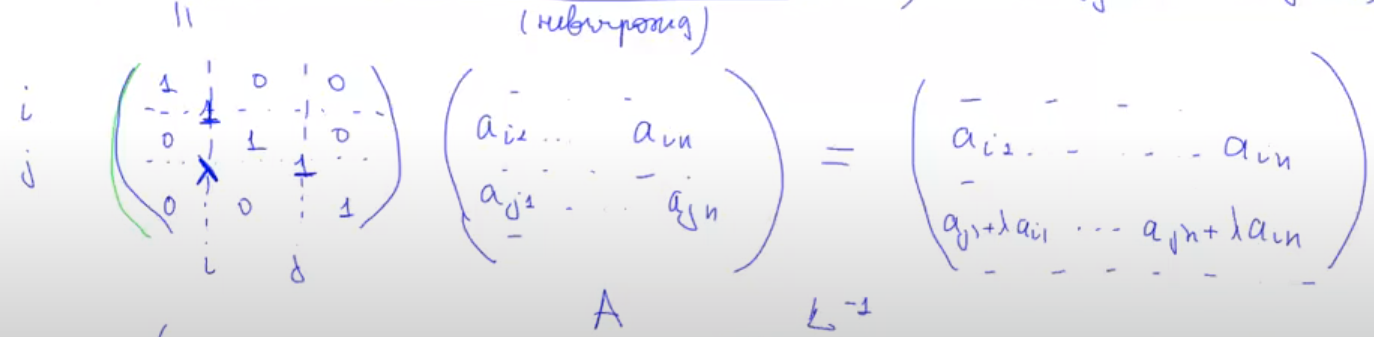
\includegraphics[width=\textwidth]{pic31}\n 
	$(\underset{\text{''прямой ход''}}{\underbracket{L_m \underbracket{\ldots \underbracket{L_1 A}}}} = DU \Space | \; \; \overbracket{L_m \ldots L_1 E}^{L^{-1}}) \Sspace \begin{matrix}
		L_m \ldots L_1 = L^{-1} \\
		(L_m \ldots L_1)^{-1} = L \n 
		\boxed{L_1^{-1} \ldots L_m^{-1} = L}
	\end{matrix} \n 
	L_i$ -- элемент нижнетреугольн.\n
	$L_m \ldots L_1 A = DU \\
	L = L_1^{-1} \ldots L_m^{-1} \Space \boxed{LDU = L_1^{-1} \underbracket{\ldots \underbracket{L_m^{-1} L_m}_E \ldots}_E L_1 A = A}\n 
	(A|E) \leadsto (\underbrace{L_m \ldots L_1}_{DU} A | \underbrace{E L^{-1}_1 L^{-1}_2 \ldots L_m^{-1}}_L)$\n 
	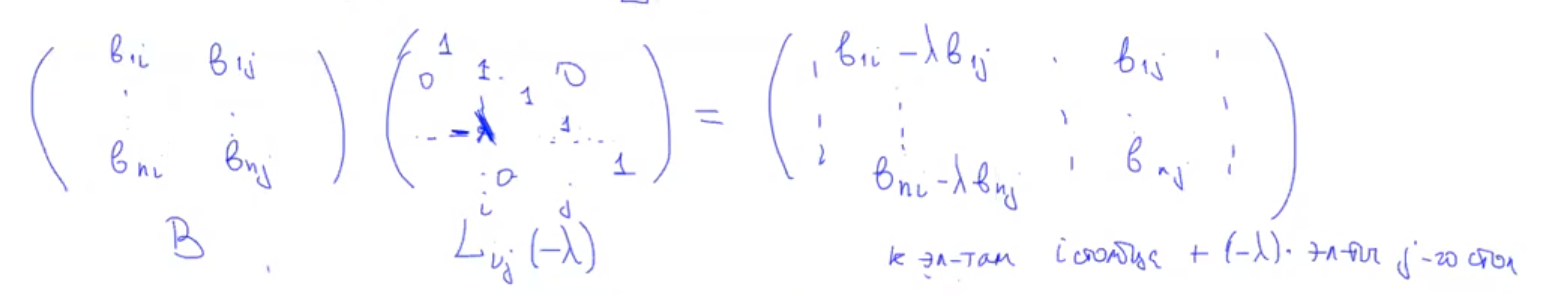
\includegraphics[width=\textwidth]{pic32}\n 
	\underline{Алгоритм}: (к j-й стр. $A + (\lambda)\cdot i$ стр. $A$ | i столб. $+ (-\lambda) \cdot j$ столб)\n 
	\begin{examples}
		$A = \begin{pmatrix}
			3 & 2 & 2 \\ 2 & 3 & -1 \\ 2 & -1 & 0
		\end{pmatrix} \Space LDU? (LU)\n 
		\triangle_1 = 3 \Space \triangle_2 = 5 \Space \triangle_3 = -4 - 4 - 12 - 3 = -23 \neq 0\n 
		\begin{pmatrix}
			\begin{matrix}
				3 & 2 & 2 \\2 & 3 & -1 \\ 2 & -1 & 0
			\end{matrix} & \vline & \begin{matrix}
				1 & 0 & 0\\0 & 1 & 0\\0 & 0 & 1
			\end{matrix}
		\end{pmatrix} \leadsto \begin{pmatrix}
			\underbracket{\begin{matrix}
					3 & 2 & 2\\0 & 5/3 & -7/3\\0 & 0 & -23/5
				\end{matrix}}_{DU} & \vline & \underbracket{\begin{matrix}
					1 & 0 & 0\\2/3 & 1 & 0\\2/3 & -7/5 & 1
				\end{matrix}}_L
		\end{pmatrix} \n U = \begin{pmatrix}
			1 & 2/3 & 2/3\\
			0 & 1 & -7/5\\
			0 & 0 & 1
		\end{pmatrix} \Space D = diag(\underset{=\triangle_1}{3}, \underset{=\frac{\triangle_2}{\triangle1}}{5/3}, \underset{= \frac{\triangle_3}{\triangle_2}}{-23/5})\n 
		A = LDU = \begin{pmatrix}
			1 & 0 & 0\\2/3 & 1 & 0\\2/3 & -7/5 & 1
		\end{pmatrix} \begin{pmatrix}
			3 & 0 & 0\\0 & 5/3 & 0\\0 & 0 & -23/5
		\end{pmatrix} \underset{=U}{\begin{pmatrix}
			1 & 2/3 & 2/3\\0 & 1 & -7/5\\0 & 0 & 1
		\end{pmatrix}} = LDL^* = U^* D U\n 
		A = A^*$
	\end{examples}
	\begin{defin}
		$\A \in End(V) \Space V$ унит. (евкл.) $\Space (\cdot, \cdot)\n 
		\A = \A^*$ самосопр.\n
		---\ \underline{положит.(отрицат.) определен}, если $\forall u \neq \0 \Space (\A u, u) \underset{(<0)}{> 0 }\  \Leftrightarrow \underset{(<0)}{\A > 0}$\n 
		--- \ \underline{положит. (отриц.) полуопред.}, если $\forall u \neq \0 \Space (\A u, u) \underset{\leq 0}{\geq 0} \ \Leftrightarrow \underset{\leq 0}{\A \geq 0}$\n 
		--- \ \underline{неопредел.}, если $\exists u, v: \Space \begin{matrix}
			(\A u, u) > 0\\
			(\A v, v) <0
		\end{matrix} \Leftrightarrow \A <>0$
	\end{defin}
	\begin{remark}\ 
		\begin{mylist}
			\item $\A > 0 \Leftrightarrow (\A u, u) \geq 0$, причем $= 0 \Leftrightarrow u = 0$\n 
			если $u = 0$, то очевидно,$\ (\A u, u) = 0$
			\item $\A = \A^* \Space (\A u, u) = (u, \A u)$
			\item 
			\begin{stat}
				$\ \\
				\begin{matrix}
					\underset{(<0)}{\A > 0} \Leftrightarrow \text{ все с.ч. } \underset{(<0)}{\lambda > 0}\n 
					\underset{(\leq 0)}{\A \geq 0} \Leftrightarrow \text{ все с.ч. }
					\underset{(\leq 0)}{\lambda \geq 0} 
				\end{matrix} \Sspace \A <> 0 \Leftrightarrow \exists$ с.ч. $\lambda, \mu: \begin{matrix}
					\lambda > 0 \\
					\mu < 0
				\end{matrix}$
			\end{stat}
			\begin{proof}
				$\A$ самосопр. $\Leftrightarrow \underset{\lambda \text{ вещ.}}{\A}$ о.п.с. $\Space V = \underset{\stackrel{\lambda}{\text{вещ. с.ч.}}}{\bigoplus} \underset{\text{собств. подпр.}}{V_\lambda} \Space \underset{\lambda \neq \mu}{V_\lambda \perp V_\mu}\n 
				\forall u \in V : u = \sum \limits_\lambda \overset{\in V_\lambda}{v_\lambda}\n 
				(\A u, u) = (\sum\limits_\lambda \A v_\lambda, \sum\limits_\mu v_\mu) = \sum\limits_\lambda \sum \limits_\mu (\lambda v_\lambda, v_\mu) = \sum\limits_\lambda \sum\limits_\mu \lambda (\underset{= 0 \ \lambda \neq \mu}{v_\lambda, v_\mu}) = \sum\limits_\lambda \lambda (\underset{>0 \text{ если } v_\lambda \text{ с.в.}}{v_\lambda, v_\lambda})\n 
				(\Leftarrow) \; \; \pu$ все $\lambda > 0 \underset{u \neq \0}{\Rightarrow} (\A u, u) = \sum \lambda (\overset{\geq 0}{v_\lambda, v_\lambda}) > 0 \Sspace \text{т.к. }\exists \lambda_0 : \; \; \underset{>0}{\lambda_0} (\underset{>0}{v_{\lambda_0}, v_{\lambda_0}}) > 0 \; \; \; v_{\lambda_0} \text{ с.в. } \neq \0\n 
				(\Rightarrow) \; \; \underset{\A > 0}{\overset{\neq \0}{v_\lambda} \text{ с.в.}} \; \; (\underset{> 0}{\A v_\lambda, v_\lambda}) = \lambda (\underset{>0}{v_\lambda, v_\lambda}) > 0 \Rightarrow \lambda > 0$
			\end{proof}
		\item Все $def$ из замечаний 1, 2, 3 переносятся на самосопряженные матрицы (симм., эрмитовы) $A = A^*\n 
		\forall x \in \R^n (\mathbb C^n)\n 
		\begin{matrix}
			(A x, x) &=& x^T A^T \vec x\\
			||\\
			(x, Ax) &=& x^T \ \vec A\  \vec x
		\end{matrix} \Space \begin{matrix}
			A > 0 \; \; \forall x \neq 0 \\
			x^T A^T \vec x > 0\\
			||\\
			x^T \vec A \vec x \text{ и т.д.}
		\end{matrix}$
		\end{mylist}
	\end{remark}
	\begin{theorem}[разложение Холецкого или метод квадратного корня]
		\ \\
		$\forall A > 0$, т.ч. $\triangle_k \neq 0 \; \; \forall k = 1 \ldots \dunderline{n} \Space \begin{matrix}
			\exists! L \text{ нижнетреуг. (причем } l_{ii} > 0)\\
			\exists! U \text{ верхнетруг. (причем } u_{ii} > 0)
		\end{matrix} \n 
		\boxed{A = L^* = U^* U}$
	\end{theorem}
	\begin{proof}
		$A = A^* \underset{\text{по следствию}}{\Rightarrow} \exists! \; \; \; A = \underset{\stackrel{\uparrow}{\text{унитреуг. нижн.}}}{L_0} D L^*_0 = U^*_0 D \underset{\stackrel{\uparrow}{\text{унитр. верх.}}}{U_0}\n 
		\forall x \neq \0 \Space 0 < (A x, x) = (L_0 D L^*_0, x) = (D \underbracket{L_0^*}_y, \underbracket{L^*_0 x}_y) = \underset{D = diag(d_1 \ldots d_n)}{(D y, y)} = d_1 y_1^2 + d_2 y^2_2 + \ldots + d_n y^2_n\n 
		\Rightarrow \begin{matrix}
			L_0 \text{ невырожд.}\\
			\left.\begin{array}{c}L^*_0 \text{ невыр.}\\ x \neq \0\end{array}\right\}
		\end{matrix} \Rightarrow \underset{= y}{L^*_0} x \neq \0$\n 
		Будем брать $y = e_j$ канон. базиса $\Rightarrow d_j < 0 \; \; \; j = 1 \ldots n \Rightarrow \n 
		\Rightarrow D = \sqrt D \sqrt D \Sspace \sqrt D:= diag(\sqrt{d_1} \ldots \sqrt{d_n})\n 
		A = \underbracket{L_0 \sqrt{D}}_L \underbracket{\sqrt{D} L^*_0}_{L^*} = \underbracket{U^*_0 \sqrt D}_{U^*} \underbracket{\sqrt D U_0}_U \Sspace L^* = (L_0 \sqrt D)^* = (\sqrt D)^* L_0 = \sqrt D L^*_0\n 
		l_{ii} = \sqrt{d_i} > 0 \slide{70px} u_{ii} = \sqrt{d_i} > 0$ \slide{100px} Аналогично $U^*\n 
		\slide{200px} (\sqrt D U_0)^* = U^*_0 \sqrt D$
	\end{proof}
\end{document}